\chapter{从当前状态到区间相对运动：IMU预积分}

\label{chap:md-10}

第八、九章围绕当前名义状态展开：IMU每来一个样本，ESKF就预测一次，再等待外部观测修正。后端面对的是另一种问题。若只优化相隔数十或数百个IMU样本的关键帧，能否先把中间的读数整理成一份长度固定、以后可以反复评价的区间记录？

预积分为这件事服务。它在固定的偏置线性化点扫描区间IMU，保存相对旋转、相对速度、相对位置、局部协方差和偏置敏感度。优化器调整两端状态时，重新比较端点预测与这份记录；小幅偏置改变先用Jacobian修正，大幅改变才重新扫描。本章先看清三种相对量，再追踪递推、误差、偏置和因子残差。

\section{从估计当前状态转向保存一段运动}

到这里，ESKF已经连贯走完。仍然看同一台机器人，只是现在后端希望同时调整多个关键帧：新的视觉观测可能让起点位置、速度、姿态都发生变化。我们需要把两帧之间的IMU信息保留下来，让这些变化能反复接受同一段数据的检验。

设关键帧时刻为$t_i<t_j$，其间的IMU样本按时间排列为

\begin{equation*}
u_k=(\omega_{m,k},a_{m,k}),\qquad
 \mathcal I_{ij}=(u_i,\ldots,u_{j-1}),\qquad
 \Delta t_k=t_{k+1}-t_k.
\end{equation*}

这里用有序序列而不是无序集合：旋转的乘法顺序会影响结果。若关键帧时刻不恰好落在IMU采样时刻，应先做时间对齐与相应插值，确定实际采用的积分区间。

ESKF给定当前名义状态后向前传播。窗口优化则同时把多个关键帧状态作为未知量，一次视觉观测可能要求修改起点姿态$R_i$，这又会改变比力投到世界系的方向。如果保存的是从旧初值出发的绝对轨迹，每次修改起点后都可能需要重新扫描同一段IMU。

预积分把这段扫描的结果写成相对测量。当$R_i,p_i,v_i$改变时，区间内递推可以复用，只重新计算端点残差；偏置的变化仍会影响预积分，需要一阶修正或重新积分。它节省的是优化迭代中对同一批高频样本的重复处理。

这里"预"表示在端点状态反复调整之前，先扫描一次区间数据；"积分"表示把许多小时间步的运动积累起来。它仍保留对偏置、时间戳和标定参数的依赖，不能理解为完全不依赖任何估计量。

与前面每一步的$h=\Delta t_k$不同，$T_{ij}=t_j-t_i$表示整段时长。起点$i$固定，$k$沿区间内的高频样本向前走，$j$是终点。后面带下标$(i,k)$的量都是"从同一个起点累积到当前采样时刻"的结果。

\section{先定义要保存的三个相对量}

以下先定义真实端点之间应有的相对量，暂时不问带噪IMU怎样算它。记$T_{ij}=t_j-t_i$，起点机体系为$B_i$，终点机体系为$B_j$。$R_i,R_j$分别把这两个机体系的向量坐标送到世界系$W$。

\begin{center}
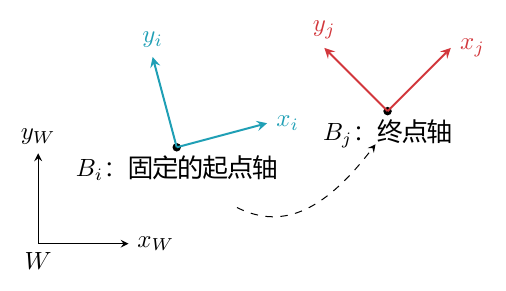
\includegraphics[width=.72\textwidth]{assets/images/附件-tikz-7-2.png}
\end{center}

预积分中的速度和位置向量始终用出发时的轴$B_i$表达。机器人之后转了多少，$B_i$这组参考轴也不跟着当前时刻的机体系一起转。图用平面坐标示意这个关系，三维情况只多一个轴。

\subsection{旋转：把终点机体系表达在起点机体系中}

固定$t_i$，记$\tau=t-t_i$，定义

\begin{equation*}
\Delta R_i(t)=R_i^\top R(t).
\end{equation*}

它把时刻$t$机体系中的向量坐标变换到起点机体系$B_i$。

用一个实际向量检验乘法方向：若它在当前机体系中的坐标为$u_t$，则

\begin{equation*}
u_t\xrightarrow{\ R(t)\ }u_W
     \xrightarrow{\ R_i^\top\ }u_i,
 \qquad u_i=R_i^\top R(t)u_t.
\end{equation*}

因此相对旋转必须写成$R_i^\top R(t)$。它先把输入送到世界系，再送回起点机体系；不是凭记忆选择矩阵的排列。 反过来左乘$R_i$，得到

\begin{equation*}
R(t)=R_i\Delta R_i(t).
\end{equation*}

两次旋转通过群乘法比较，不能用$R(t)-R_i$代替相对旋转。

\subsection{速度：扣除初速与重力，再改变表达坐标}

如果只算$v(t)-v_i$，里面还包含已知重力在$\tau$时间内产生的速度变化$g_W\tau$。我们希望把这部分留给重建公式单独处理，于是先扣掉它，再换到$B_i$。

定义

\begin{equation*}
\Delta v_i(t)=R_i^\top(v(t)-v_i-g_W\tau).
\end{equation*}

先取速度变化$v(t)-v_i$，扣除已知重力产生的$g_W\tau$，再用$R_i^\top$把剩余量表达在$B_i$。重建速度时反向操作：

\begin{equation*}
v(t)=v_i+g_W\tau+R_i\Delta v_i(t).
\end{equation*}

$\Delta v_i$的单位仍然是速度，但它并非世界系的$v(t)-v_i$。

\subsection{位置：扣除初始位置、初速位移与重力位移}

同样，从$p(t)$中逐项剥离：第一步减$p_i$，得到从出发点到当前点的位移；第二步减$v_i\tau$，去掉即使没有加速度也会产生的位移；第三步减$\tfrac12g_W\tau^2$，去掉重力的解析贡献；最后才用$R_i^\top$改变表达坐标。

定义

\begin{equation*}
\Delta p_i(t)=R_i^\top
       (p(t)-p_i-v_i\tau-\tfrac12g_W\tau^2).
\end{equation*}

重建时反向操作，先乘回$R_i$，再把三个扣除项加回来：

\begin{equation*}
p(t)=p_i+v_i\tau+\tfrac12g_W\tau^2+R_i\Delta p_i(t).
\end{equation*}

由定义可知$\Delta R_i(t_i)=I$、$\Delta v_i(t_i)=0$、$\Delta p_i(t_i)=0$。在$t_j$记$T_{ij}=t_j-t_i$，三条端点重建关系为

\begin{equation}\label{eq-preint-reconstruction}
\boxed{
\begin{aligned}
 R_j&=R_i\Delta R_{ij},\\
 v_j&=v_i+g_WT_{ij}+R_i\Delta v_{ij},\\
 p_j&=p_i+v_iT_{ij}+\tfrac12g_WT_{ij}^2+R_i\Delta p_{ij}.
\end{aligned}}
\end{equation}

$\Delta v$和$\Delta p$都在固定的$B_i$表达，不在不断变化的当前机体系中。

三条重建公式是本章的中心。预积分先保存右边的相对运动，使用时再乘回$R_i$、加回起点速度与位置以及重力项。每条定义都能通过这个逆操作检查：左乘$R_i$，利用$R_iR_i^\top=I$，然后把先前扣掉的项移回去。

\begin{bookexample}{自由落体与静止的预积分有什么不同}

理想自由落体中，比力$a=0$。若没有转动，重建所需的相对量是$\Delta R=I,\Delta v=0,\Delta p=0$，所有世界系速度和位置变化都由显式重力项提供。

静止在桌上的IMU则受到支撑，比力为$-R_i^\top g_W$。此时预积分的速度和位置量并不为零，它们恰好在重建时抵消重力贡献。下文会用连续积分再次检查这一点。

\end{bookexample}

\section{用IMU逐步算出这段相对运动}

\subsection{理想关系怎样成为可计算的量}

刚才的$\Delta R,\Delta v,\Delta p$由真实状态定义，说明我们要保存什么；实际计算只有带噪声的IMU读数。因此先选定偏置$\bar b_g:=\bar b_{g,i}$、$\bar b_a:=\bar b_{a,i}$，在本次区间扫描中固定使用它们。横线表示\textbf{这一次预积分的偏置线性化点}，它不必等于最终优化得到的偏置。

用这些偏置扣除读数，仍将采用的输入记为

\begin{equation*}
\hat\omega_k=\omega_{m,k}-\bar b_g,\qquad
 \hat a_k=a_{m,k}-\bar b_a.
\end{equation*}

与ESKF每步使用当前偏置估计相比，此处整段扫描固定在$\bar b_g,\bar b_a$。由它们算出的结果加波浪线，表示\textbf{已经由读数计算出的名义预积分量}，不表示精确真实值或精确统计均值。

从固定相对初值开始：

\begin{equation*}
\widetilde{\Delta R}_{i,i}=I,\qquad
 \widetilde{\Delta v}_{i,i}=0,\qquad
 \widetilde{\Delta p}_{i,i}=0.
\end{equation*}

这一瞬间还没有积累运动，与机器人在世界系中的初始位置和速度无关。

\subsection{三条递推分别做什么}

记$h=\Delta t_k$。对与ESKF一致的区间起点近似，三条递推为

\begin{equation}\label{eq-intuition-preint-step}
\begin{aligned}
 \widetilde{\Delta R}_{i,k+1}
 &=\widetilde{\Delta R}_{i,k}\mathop{\mathrm{Exp}}((\hat\omega_kh)^\wedge),\\
 \widetilde{\Delta v}_{i,k+1}
 &=\widetilde{\Delta v}_{i,k}+\widetilde{\Delta R}_{i,k}\hat a_kh,\\
 \widetilde{\Delta p}_{i,k+1}
 &=\widetilde{\Delta p}_{i,k}+\widetilde{\Delta v}_{i,k}h
   +\tfrac12\widetilde{\Delta R}_{i,k}\hat a_kh^2.
\end{aligned}
\end{equation}

第一式把当前小旋转接到已有相对旋转的右边：输入一个下一时刻机体系的向量，先送回当前机体系，再送回固定的$B_i$。所以时间推进时在右边接新因子，不能任意颠倒乘法。

第二式先用$\widetilde{\Delta R}_{i,k}$把当前比力送到$B_i$，再乘时间累加。不同采样时刻的传感器轴可能不同，经过这一步才可以把各次读数加在同一组方向上。

第三式同时保留已积累的相对速度继续产生的位移，以及本步比力带来的二次时间项。它使用旧速度和旧旋转；三条右端一起用第$k$步旧值计算，再提交新值。这里不再加世界系重力，因为重力已由式\eqref{eq-preint-reconstruction}单独加回。

这也让第\ref{chap:md-06}章的非交换性有了具体用途：保存旋转时要按时间依次连乘小旋转，一般不能把所有角度向量相加后只取一次指数。下文会从相对量的定义求导，说明这三条递推为什么不显式依赖待优化的$R_i,p_i,v_i$。

\begin{bookexample}{用两个采样区间手算速度与位置}

只看水平分量，姿态不转，两个时间步均为$h=0.5\,\mathrm s$，去偏置后的水平比力依次为$2$和$4\,\mathrm{m/s^2}$。从$\widetilde{\Delta v}=0,\widetilde{\Delta p}=0$开始，第一步得到

\begin{equation*}
\widetilde{\Delta v}_{i,i+1}=2\times0.5=1,\qquad
 \widetilde{\Delta p}_{i,i+1}=\tfrac12\times2\times0.5^2=0.25.
\end{equation*}

第二步使用第一步结束时的旧速度$1$：

\begin{equation*}
\widetilde{\Delta v}_{i,i+2}=1+4\times0.5=3,
\end{equation*}

\begin{equation*}
\widetilde{\Delta p}_{i,i+2}
 =0.25+1\times0.5+\tfrac12\times4\times0.5^2=1.25.
\end{equation*}

速度单位为$\mathrm{m/s}$，位置单位为$\mathrm m$。如果只把两步的$\tfrac12ah^2$相加，会得到$0.75$，漏掉早期加速度所产生的速度在第二步中继续带来的$0.5$位移。

若起点水平位置为$10$、速度为$3$，总时长为$1$，则重建的终点为$v_j=6$、$p_j=14.25$。保存的预积分量是$3$与$1.25$，使用起点后才得到这两个世界系终点值。

\end{bookexample}

\section{保存相对运动时，也保存不确定性与偏置敏感度}

\subsection{相对量也有自己的局部误差}

读数有噪声，算出的相对运动当然也会偏离理想值。沿用同一套局部误差思想：

\begin{equation*}
\begin{aligned}
 \Delta R_{i,k}&=\widetilde{\Delta R}_{i,k}\mathop{\mathrm{Exp}}(\delta\theta_{i,k}^\wedge),\\
 \Delta v_{i,k}&=\widetilde{\Delta v}_{i,k}+\delta v_{i,k},\\
 \Delta p_{i,k}&=\widetilde{\Delta p}_{i,k}+\delta p_{i,k}.
\end{aligned}
\end{equation*}

把误差按计算链条排列为

\begin{equation*}
e_{i,k}=(\delta\theta_{i,k}^\top,\delta v_{i,k}^\top,
              \delta p_{i,k}^\top)^\top\in\mathbb R^9,
 \qquad\Sigma_{i,k}=\operatorname{Cov}(e_{i,k}).
\end{equation*}

$\Sigma$描述这一段\textbf{相对测量}的不确定性，ESKF的$P$描述\textbf{当前状态}的不确定性。二者参考对象不同。此处误差顺序为$(\theta,v,p)$；速度和位置沿固定$B_i$表达，旋转误差坐标由右侧扰动关系确定。

\subsection{同一个传播原理，用在不同对象上}

先固定区间偏置，仅考虑测量噪声。将本步陀螺和加速度计的离散噪声合为$\eta_k$，其协方差记为$Q_k$。名义递推附近的一阶误差关系为

\begin{equation*}
e_{i,k+1}\simeq F_ke_{i,k}+G_k\eta_k.
\end{equation*}

$F_k$把已有相对误差送到下一步，$G_k$把当前噪声送进相对误差。它们是式\eqref{eq-intuition-preint-step}对应一步映射的微分；下文说明其中几个主要耦合块。因此

\begin{equation}\label{eq-intuition-sigma}
\boxed{\Sigma_{i,k+1}=F_k\Sigma_{i,k}F_k^\top+G_kQ_kG_k^\top,
 \qquad\Sigma_{i,i}=0.}
\end{equation}

起点相对量固定为$(I,0,0)$，还没有积累区间噪声，所以从零协方差开始。不能把ESKF起点的$P_i$填进这里；起点状态的不确定性由后端的状态变量与先验另行描述。

陀螺噪声先改变相对旋转，再改变比力的投影，随后影响速度和位置。同一次加速度噪声也同时进入速度与位置。因此$\Sigma$要保存这些相关性，不能仅记录三组互不相关的误差大小。形式$F\Sigma F^\top$仍然是局部微分之后的二阶矩传播，没有换用另一套概率原理。

若还允许偏置在区间内随机游走，就把$e$扩为十五维，按$(\theta,v,p,b_g,b_a)$排列，协方差记为$\Sigma^{(15)}$，同样从零开始累积。它同时记录区间运动误差、偏置增量以及二者相关性。后面的完整IMU因子使用这一份联合协方差；具体十五维噪声块须随所选偏置演化模型一起构造。

\subsection{为什么保存了积分，偏置改变后仍要修正}

起点位置、速度和姿态已从递推中消去，但去偏置输入仍依赖$\bar b_g,\bar b_a$。优化器若认为偏置应略大一些，同一批读数中应扣掉的量就更多，原先算出的运动也要相应改变。

记当前起点偏置与保存值之差为

\begin{equation*}
\delta b_g=b_{g,i}-\bar b_g,\qquad
 \delta b_a=b_{a,i}-\bar b_a.
\end{equation*}

这里的$\delta b$是优化候选值相对线性化点的差；它与前面未知的随机偏置误差作用不同。我们在扫描IMU时一并保存五个敏感度矩阵：$J_{R g},J_{v g},J_{v a},J_{p g},J_{p a}$。下标前一项指出哪个积分量会变化，后一项指出改变哪类偏置。例如$J_{v g}\delta b_g$回答"陀螺偏置改变这一点，整段速度积分约变化多少"。每个块都是$3\times3$。

这就是第\ref{chap:md-05}章微分的另一种用法：固定同一批输入数据，对积分计算中采用的偏置求导。旋转对加速度计偏置没有依赖，因此这里只有五个块；陀螺偏置则会通过旋转影响全部三个量。

用上标$c$表示按当前偏置修正后的测量：

\begin{equation}\label{eq-intuition-bias-correction}
\begin{aligned}
 \Delta R_{ij}^{c}
 &=\widetilde{\Delta R}_{ij}\mathop{\mathrm{Exp}}((J_{R g,ij}\delta b_g)^\wedge),\\
 \Delta v_{ij}^{c}
 &=\widetilde{\Delta v}_{ij}+J_{v g,ij}\delta b_g+J_{v a,ij}\delta b_a,\\
 \Delta p_{ij}^{c}
 &=\widetilde{\Delta p}_{ij}+J_{p g,ij}\delta b_g+J_{p a,ij}\delta b_a.
\end{aligned}
\end{equation}

速度和位置通过加法修正，旋转通过右侧小旋转修正。这些都是原偏置附近的一阶近似；偏置改变较大时，需要在新偏置处重新扫描IMU，并更新敏感度和协方差。小修正时沿用原协方差，也是围绕原线性化点的近似。

\begin{bookexample}{给刚才的两步运动多扣一点偏置}

两步水平比力仍为$2$和$4$，各持续$0.5\,\mathrm s$，总时长为$1$。如果新偏置比原值大$0.1\,\mathrm{m/s^2}$，两步采用的输入就变成$1.9$和$3.9$。原来的$\widetilde{\Delta v}=3$、$\widetilde{\Delta p}=1.25$分别变成$2.9$与$1.20$。

这里不转动，该方向的敏感度为$J_{v a}=-T_{ij}=-1$、$J_{p a}=-\tfrac12T_{ij}^2=-0.5$。乘以偏置变化$0.1$，恰好得到$-0.1$与$-0.05$的修正。这一例子中关系是线性的，三维转动时保存的Jacobian给出的是局部近似。

\end{bookexample}

\section{把两份运动描述比较成优化约束}

\subsection{端点状态说了什么，IMU又说了什么}

现在已经有两份关于同一区间的描述。一份来自当前正在优化的$x_i,x_j$：按相对量定义扣除初值与重力，得到候选状态认为发生的运动。另一份来自已扫描过的IMU：使用式\eqref{eq-intuition-bias-correction}得到按当前偏置修正后的运动测量。

速度和位置在同一个$B_i$中表达，直接相减即可；旋转要先比较群元素，再取局部对数。因此定义

\begin{equation}\label{eq-intuition-imu-residual}
\begin{aligned}
 r_R&=\mathop{\mathrm{Log}}\bigl((\Delta R_{ij}^{c})^\top R_i^\top R_j\bigr)^\vee,\\
 r_v&=R_i^\top(v_j-v_i-g_WT_{ij})-\Delta v_{ij}^{c},\\
 r_p&=R_i^\top(p_j-p_i-v_iT_{ij}-\tfrac12g_WT_{ij}^2)-\Delta p_{ij}^{c}.
\end{aligned}
\end{equation}

旋转一致时，$\mathop{\mathrm{Log}}$里面为$I$，因而$r_R=0$；速度和位置一致时，对应两个差也为零。$r_R$是三维局部旋转坐标，$r_v$的单位是速度，$r_p$的单位是位置。

这里使用"端点预测减预积分测量"的方向。前面的滤波创新$r=z-\hat z$使用"观测减预测"；两种定义各自与后续公式配套。读公式时先分清它正在比较哪两个对象。

\begin{bookexample}{用前面的两个采样区间检查残差}

接着上一节偏置增加$0.1$的情形，修正后测量为$\Delta v^c=2.9$、$\Delta p^c=1.20$，$T_{ij}=1$，起点仍为$p_i=10,v_i=3$。若当前端点估计为$v_j=6.1,p_j=14.45$，则

\begin{equation*}
r_v=(6.1-3)-2.9=0.2\,\mathrm{m/s},
\end{equation*}

\begin{equation*}
r_p=(14.45-10-3\times1)-1.20=0.25\,\mathrm m.
\end{equation*}

状态估计认为比修正后的IMU测量多增加了$0.2$速度、$0.25$额外位移。把终点改为$v_j=5.9,p_j=14.20$，这两个残差都为零。这样，偏置的改变通过预积分修正，最终传到了端点约束中。

如果只把起点速度增加$0.1$，速度与位置残差都会变化，因为它同时出现在$v_j-v_i$和$p_j-p_i-v_iT_{ij}$中；这正是端点Jacobian需要反映的耦合关系。

\end{bookexample}

若采用偏置随机游走，还要比较两端偏置，定义

\begin{equation*}
r_{b_g}=b_{g,j}-b_{g,i},\qquad r_{b_a}=b_{a,j}-b_{a,i}.
\end{equation*}

它们表达偏置随区间演化的偏离，与当前偏置相对$\bar b$的修正量不同。将完整残差按旋转、速度、位置、陀螺偏置、加速度计偏置的顺序排列：

\begin{equation*}
r_{ij}^{\mathrm{IMU}}
 =(r_R^\top,r_v^\top,r_p^\top,r_{b_g}^\top,r_{b_a}^\top)^\top.
\end{equation*}

这十五个数共同接受$\Sigma^{(15)}_{ij}$的加权，其中运动与偏置之间的相关性也被保留。

\subsection{协方差说明多大的差才值得在意}

假设某方向残差为$0.1\,\mathrm m$。若其标准差为$0.01\,\mathrm m$，这个差已经有十个标准差；若标准差为$0.2\,\mathrm m$，它只相当于半个标准差。单看残差数值，不能判断数据与状态是否相容。

在局部高斯模型下，简记$r_{ij}=r_{ij}^{\mathrm{IMU}}$，因子权重与

\begin{equation*}
\psi_{ij}(x_i,x_j)\propto
 \exp\left[-\tfrac12r_{ij}^\top(\Sigma^{(15)}_{ij})^{-1}r_{ij}\right]
\end{equation*}

对应。$\psi_{ij}$是在固定这段IMU数据后，评价两端候选状态相容程度的函数。协方差在当前优化中固定、正定时，取负对数得到代价

\begin{equation}\label{eq-intuition-factor-cost}
\boxed{E_{ij}=\tfrac12r_{ij}^\top(\Sigma^{(15)}_{ij})^{-1}r_{ij}.}
\end{equation}

这既按照各方向的不确定性缩放，也处理分量之间的相关性。若写成$\Sigma^{(15)}_{ij}=LL^\top$，求解$L\widetilde r_{ij}=r_{ij}$就得到白化残差，代价等于$\tfrac12\|\widetilde r_{ij}\|^2$。这是有相关性时"除以标准差"的对应操作。

第\ref{chap:md-07}章在这里提供了从概率到权重的依据：选定局部高斯误差模型，才能得到这种二次代价。它是局部近似，不能把一个点处的密度数值直接理解为"真实状态恰好在这里的概率"。

\subsection{后端怎样使用这份约束}

把窗口中所有关键帧合称为$X$。在相应条件独立假设下，先验、视觉和IMU因子的概率权重相乘，负对数就成为代价相加：

\begin{equation*}
X^*=\arg\min_X\left(E_{\mathrm{prior}}(X)
       +\sum_{(i,j)}E_{ij}^{\mathrm{IMU}}(X)
       +\sum_a E_a^{\mathrm{visual}}(X)\right).
\end{equation*}

$E_{\mathrm{prior}}$保存已有信息，视觉项比较图像测量，IMU项比较相邻关键帧间的运动。优化器寻找一组能共同解释这些数据的状态。

改变端点会改变残差。在当前$X$附近写

\begin{equation*}
r(X\oplus\delta X)\simeq r(X)+J\delta X.
\end{equation*}

这里$\delta X$是所有关键帧的局部增量，$J$把状态增量送到残差变化。后端在这个局部关系上计算能减小加权误差的增量，再用$\oplus$更新状态。第\ref{chap:md-05}章的微分和第\ref{chap:md-06}章的合法状态更新，又在这里接到一起。本章后面给出端点残差的主要Jacobian块；多个因子怎样共同组成优化方程留到第\ref{chap:md-12}章。

端点位置、速度、姿态改变时，重新计算的是式\eqref{eq-intuition-imu-residual}这一侧；已保存的区间预积分可以复用。当前偏置改变时，先用保存的敏感度修正；变化较大才重新积分。这就完成了预积分从输入数据到优化用途的整条链。

\section{从相对定义到递推：检查最重要的三条微分}

\subsection{固定起点，再对当前时刻求导}

令$\tau=t-t_i$，将本章前面定义的三个相对量看成$t$的函数：

\begin{equation*}
\Delta R_{it}=R_i^\top R_t,\quad
\Delta v_{it}=R_i^\top(v_t-v_i-g_W\tau),\quad
\Delta p_{it}=R_i^\top(p_t-p_i-v_i\tau-\tfrac12g_W\tau^2).
\end{equation*}

求导时$R_i,p_i,v_i$属于固定的起点参数。利用$\dot R_t=R_t\omega_t^\wedge$及$\dot v_t=g_W+R_ta_t$，得到

\begin{equation*}
\dot{\Delta R}_{it}=\Delta R_{it}\omega_t^\wedge,\qquad
\dot{\Delta v}_{it}=\Delta R_{it}a_t,\qquad
\dot{\Delta p}_{it}=\Delta v_{it}.
\end{equation*}

起点值为$(I,0,0)$。这三式说明：初始世界系位置、速度和重力已经由相对量定义扣除；积分时只需按起点机体系累积角速度与比力。把每个采样间隔中的输入近似固定，就得到前面的离散递推。有关流形预积分的经典推导可对照\href{https://arxiv.org/abs/1512.02363}{Forster等人的论文}；本笔记仍以已经约定的区间起点积分器为准。

\subsection{较早的加速度为什么影响位置更久}

由于$\dot{\Delta p}=\Delta v$，某次比力先改变相对速度，改变后的速度又在余下区间不断累积为位移。连续写法中，一个时刻$s$的加速度对终点位置带有剩余时间$t_j-s$的权重；离散递推则通过“旧$\Delta v$乘本步时长”体现同一事实。这个观察比直接记住位置递推中的一串求和更容易检查符号和时间因子。

\section{一步误差微分怎样形成协方差递推}

\subsection{姿态误差怎样进入速度和位置}

本章使用右侧旋转误差。若当前相对旋转略有偏差$\delta\theta$，加速度投影的一阶变化满足

\begin{equation*}
\Delta R\operatorname{Exp}(\delta\theta^\wedge)\hat a
\simeq\Delta R\hat a-\Delta R\hat a^\wedge\delta\theta.
\end{equation*}

因此一步速度映射关于旧姿态误差的块包含$-\Delta R\hat a^\wedge h$；位置映射中相应块含$\tfrac12h^2$。旧速度误差还通过$h\,\delta v$进入新位置。这里给出的是这几个容易在实现中漏掉的耦合，完整$F_k,G_k$仍须对实际采用的同一张离散映射求导。

\subsection{噪声先进入哪一个量}

陀螺噪声直接扰动单步旋转，然后借由后续的比力投影间接影响速度和位置；加速度计噪声在当前步直接进入速度和位置。即使同一次测量噪声只来自几个独立通道，积分后的旋转、速度和位置误差也可能相关。若把所有交叉协方差强行设为零，后端便会失去“这几项误差来自同一批IMU读数”的信息。

\subsection{连续噪声密度不能直接当作单步协方差}

第九章已经区分连续白噪声谱密度与有限时间噪声增量。预积分使用同一批传感器参数，但$\Sigma_{ij}$从区间起点的零值开始累积，$P_i$则是当前状态估计已有的不确定性。若采用区间平均噪声样本，其协方差随$1/h$缩放；经一步积分映射后，位置与速度块再出现各自的时间因子。噪声模型或积分器改变时，应一起更新$G_kQ_kG_k^\top$，不能只在最终$\Sigma_{ij}$上乘一个经验常数。

\section{五个偏置Jacobian怎样随积分累积}

\subsection{陀螺偏置的影响要搬到新的右侧坐标}

记本步旋转$A_k=\operatorname{Exp}(\phi_k^\wedge)$，$\phi_k=(\omega_{m,k}-\bar b_g)h$。偏置增加$\delta b_g$使本步旋转向量变为$\phi_k-\delta b_gh$。旧区间旋转的偏置影响与新一步的直接影响，都要表达在更新后相对旋转的右侧局部坐标中，得到

\begin{equation*}
J_{Rg,i,k+1}
=A_k^\top J_{Rg,i,k}-J_r(\phi_k)h,\qquad J_{Rg,i,i}=0.
\end{equation*}

$J_r(\phi_k)$处理单步指数映射的微分，$J_{Rg,i,k}$则保存整段截至$k$的偏置敏感度。输入变量、保存时间和作用对象不同，不能混称为同一个Jacobian。

\subsection{速度与位置敏感度各走哪些路径}

速度对陀螺偏置的变化，经“偏置$\to$姿态$\to$比力方向$\to$速度”；速度对加速度计偏置的变化，直接由本步扣除的比力产生。位置还多经过“旧速度$\to$本步位移”这条路径，因此更新位置Jacobian时要使用旧速度Jacobian。五个块都从零开始，按与名义量相同的步序递推。正文保留路径和上一节的旋转代表式；逐块矩阵可在实际实现时对选定的离散递推逐项求导，不宜把另一种积分器的块直接移用过来。

\subsection{什么时候重积分}

一阶修正只在偏置线性化点附近可靠。若$ b_{g,i}-\bar b_g$或$b_{a,i}-\bar b_a$过大，或者重新标定了时间偏差、外参和噪声模型，就需要用原始IMU样本重新计算区间记录。仅替换残差中的当前偏置，不会自动使旧预积分结果与新模型一致。

\section{端点变化怎样进入IMU残差}

\subsection{先固定优化时使用的局部增量}

对$R_i,R_j$采用右侧扰动，对$p,v,b_g,b_a$采用加法。预积分记录、偏置线性化点和当前协方差先固定；优化器改变的是端点候选状态。于是端点Jacobian是第十章残差对$(\delta x_i,\delta x_j)$的局部微分，行顺序随残差$(R,v,p,b_g,b_a)$，列顺序随状态$(\theta,p,v,b_g,b_a)$。

\subsection{速度与位置残差的代表性块}

记$q_v=R_i^\top(v_j-v_i-g_WT_{ij})$，$q_p=R_i^\top(p_j-p_i-v_iT_{ij}-\tfrac12g_WT_{ij}^2)$。由于起点姿态改变时，相对向量的表达坐标改变，

\begin{equation*}
\operatorname{Exp}(-\delta\theta_i^\wedge)q
\simeq q+q^\wedge\delta\theta_i.
\end{equation*}

因此速度残差中出现$q_v^\wedge\delta\theta_i$、$-R_i^\top\delta v_i$和$R_i^\top\delta v_j$；位置残差还出现$-R_i^\top\delta v_iT_{ij}$。起点偏置的各块以负的预积分偏置Jacobian进入。$R_j$没有直接出现在当前定义的$r_v,r_p$中，它主要进入旋转残差。这个例子已经足以检查多数端点矩阵块来自哪条映射；旋转残差还需使用$\operatorname{Log}$的局部微分。

\section{一次预积分扫描与反复评价}

从$(I,0,0)$、零Jacobian和零区间协方差开始，按时间戳逐步去偏置、更新三个相对量、五个敏感度块与协方差。区间终点保存时长、偏置线性化点、三种名义相对量、敏感度和协方差；必要时保留原始IMU以供重积分。后端每次评价因子时，用当前起点偏置作一阶修正，再从两端候选状态计算预测相对量，形成残差并白化。端点位姿变化不要求重新扫描原始IMU。

\begin{center}\small\begin{tabular}{p{0.280\textwidth}p{0.280\textwidth}p{0.280\textwidth}}\toprule

所问问题 & ESKF当前状态 & 预积分区间记录 \\

\midrule

参考对象 & 当前名义状态$\hat x_t$ & 固定起点的相对测量$\widetilde\Delta_{ij}$ \\

协方差 & 已有状态误差$P_t$继续传播 & 本区间误差$\Sigma_{ij}$从零累积 \\

新数据到来时 & 继续预测并等待观测修正 & 继续累积本区间测量 \\

后端反复优化时 & 当前滤波循环本身不回放全部历史 & 用相同记录反复评价新的端点候选 \\

\bottomrule\end{tabular}\end{center}

下一章换一类输入：若不是IMU读数，而是两帧点云，该怎样从局部几何求出相对位姿？这就是GICP要解决的问题。
